\newenvironment{codeblock}{\captionsetup{type=listing}}{}
\SetupFloatingEnvironment{listing}{name=Code}

\addappheadtotoc

\begin{appendix}
\chapter{L'Interface Utilisateur}

\section{JavaFX}
\label{javafx}

JavaFX est un framework\footnote{Un framework est un ensemble d'outils permettant de développer plus facilement certaines partie d'une application, ici notre interface graphique.} pour créer des interfaces graphiques qui remplace historiquement le framework Swing, utilisé dans la première partie de ce projet pour construire l'IHM. JavaFX peut-être utilisé procéduralement\footnote{via une série d'appels de fonctions.} comme Swing pour créer l'interface graphique ou via la création d'un fichier à la syntaxe spécifique pour décrire la structure que prendra l'IHM.

On explorera dans cette annexe les concepts clés de JavaFX comme les notions de \textit{bindings} par exemple. On verra aussi comment utiliser le FXML avec l'outil \href{https://gluonhq.com/products/scene-builder/}{Scene Builder}.

\subsection{Organisation}

L'organisation d'une interface JavaFX repose sur quelques concepts particuliers que l'on retrouvera dans notre code.

\begin{figure}[p]
  \centering
  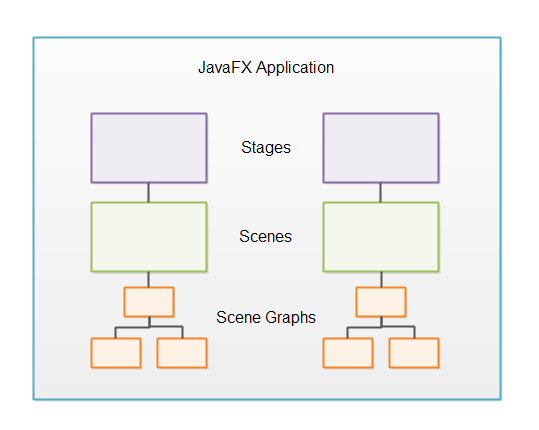
\includegraphics{./media/javafx-architecture.png}
  \caption{Architecture d'une interface JavaFX}
\end{figure}

\begin{description}
  \item [Stage] Un stage représente une fenêtre d'application. Autant de stage que nécessaire pourront être crées. Il est a noter que lors de l'initialisation de l'interface, JavaFX créera pour nous un stage nommé stage primaire.
  \item [Scene] Un stage doit contenir une unique scène qui pourra être changé au cours de l'exécution du programme. Une scène englobe ce qui sera affiché dans un stage.
  \item [Node] Les nodes sont tous les éléments composant l'interface graphique (boutons, zone de texte etc.) sont attachés a une scène. On nomme cet ensemble le graphe de la scène. 
\end{description}

\section{Base}

Pour créer une interface graphique de base en JavaFX, on doit créer une nouvelle classe qui étend \code{Application}. Ensuite, la construction de l'interface passe par la redéfinition de la méthode \code{start} qui fournira en paramètre le stage primaire (discuté un peu plus haut).

Voici un code très basique montrant la création d'un simple "Hello World" en JavaFX. 

\begin{codeblock}
\begin{minted}{java}
import javafx.application.Application;
import javafx.scene.Scene;
import javafx.scene.control.Label;
import javafx.stage.Stage;

public class HelloWorld extends Application {

    @Override
    public void start(Stage primaryStage) throws Exception {
        primaryStage.setTitle("My First JavaFX App");
        
        Label label = new Label("Hello World !");
        Scene scene = new Scene(label, 400, 200);
        primaryStage.setScene(scene);
        
        primaryStage.show();
    }

    public static void main(String[] args) {
        HelloWorld.launch(args);
    }
}
\end{minted}
\captionof{listing}{"Hello World" en JavaFX}
\end{codeblock}

Code qui, une fois exécuté dans \href{https://www.bluej.org/}{BlueJ} (qui intègre nativement le support de JavaFX), donne cette fenêtre.

\begin{figure}[ht]
  \centering
  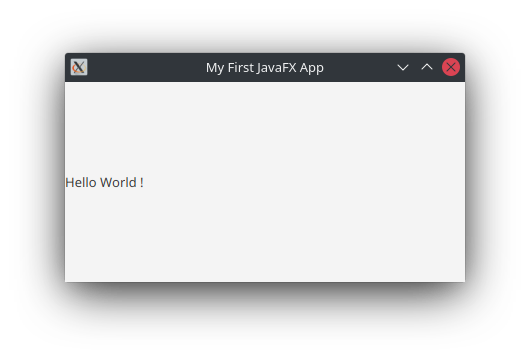
\includegraphics[width=10cm,height=10cm,keepaspectratio]{./media/first_javafx_app.png}
  \caption{Application JavaFX basique.}
\end{figure}

Le code ci-dessus ne fait rien de plus que changer le titre de notre fenêtre puis crée un nouveau \href{https://openjfx.io/javadoc/11/javafx.controls/javafx/scene/control/Label.html}{Label} qui contient le texte que nous voulons afficher. Ensuite, il nous faut une \code{Scene} pour structurer notre interface. Une fois que tous les éléments sont en place, on affiche l'objet \code{Stage} via l'appel de \code{show}.

Évidement, pour agencer plusieurs éléments (une zone de texte, des boutons, des images etc.), comme pour avec \code{Swing}, on devra se servir des différents conteneurs de JavaFX. Voici une liste (non-exhaustive) des conteneurs que vous pouvez utiliser avec \code{JavaFX}. Un conteneur permet d'imposer une certaines logiques de disposition dans l'interface à ses éléments enfants (notre fenêtre de tout à l'heure est le parent de notre \code{Scene} qui est lui-même parent de notre \code{Label}).

\begin{description}
  \item [BorderPane] Vous avez certainement dû l'utiliser avec \code{Swing} dans les premières version de l'IHM. Ce conteneur permet d'agencer les élements en 5 zones distinctes : le haut, le bas, la gauche, la droite et le centre.
  \item [HBox] Le conteneur \code{HBox} (pour Horizontal Box) agencera ses enfants à la suite horizontalement.
  \item [VBox] Le conteneur \code{VBox} (pour Vertical Box, vous ne vous y attendiez pas) agencera ses enfants à la suite verticalement.
  \item [GridPane] Ce conteneur permet une très grande liberté du placement des enfants. Il permet de diviser son espace en une grille et de donner à chaque enfants une position dans cette grille.
  \item [StackPane] Ce conteneur permet la disposition de ses enfants l'un par dessus l'autre. Le premier élement sera l'élement le plus "loin" de l'écran, le dernier ajouté sera au premier plan.
\end{description}

Pour plus de matière sur les conteneurs, n'hésitez pas à jouer avec dans Scene Builder où de regarder \href{https://openjfx.io/javadoc/11/index.html}{la documentation} de JavaFX.

\section{FXML}

La question pouvant se poser à ce niveau est la différence entre JavaFX et Swing, utilisé précédemment pour construire l'IHM, c'est ce que nous allons discuter ici.

Vous avez pu remarquer en jouant un peu avec Swing que très vite, pour complexifier l'interface du Zuul (imaginons un ajout de boutons, d'images, de zones de d'affichage voir d'autres fonctionnalités plus ou moins avancés etc.), le nombre de lignes augmentait et le code devenait de plus en plus difficile à lire et la maintenance compliquée. On peut imaginer séparer l'interface graphique en plusieurs composants mais cela demande du temps et beaucoup de rigueur.

JavaFX vient avec sa propre solution pour faciliter la construction d'interface graphique en découplant fortement la logique (le code Java donc) de l'interface graphique (qui sera définit dans un format de balisage nommé FXML). L'avantage de définir son interface en FXML est que la hiérarchie est tout de suite visible à la lecture du fichier. Regardons un exemple de code FXML pour s'en convaincre.

\begin{codeblock}
\captionof{listing}{"Hello World" en FXML}
\begin{minted}{xml}
<?xml version="1.0" encoding="UTF-8"?>

<?import java.lang.*?>
<?import java.util.*?>
<?import javafx.scene.*?>
<?import javafx.scene.control.*?>
<?import javafx.scene.layout.*?>

<AnchorPane id="AnchorPane" prefHeight="200" prefWidth="320" xmlns:fx="http://javafx.com/fxml/1" fx:controller="com.example.DocumentController">
    <children>
        <Button layoutX="126" layoutY="90" text="Click Me!" onAction="#handleButtonAction" fx:id="button" />
        <Label layoutX="126" layoutY="120" minHeight="16" minWidth="69" fx:id="label" />
    </children>
</AnchorPane>
\end{minted}
\end{codeblock}

Il apparaît directement que cette interface est basé sur un parent qui est un \code{AnchorPane} dont on repère les dimensions. Ce parent contient en enfant un bouton et une zone d'affichage de texte.

Pour créer notre propre fichier FXML avec notre interface, on peut utiliser un outil de type drag \& drop nommé Scene Builder pour concevoir facilement notre interface. Jouez un peu avec les différents élements et conteneurs.

\section{Lien entre FXML et code Java}

\section{Implémentation dans le projet Zuul}



\chapter{Les dialogues}

La plus grande particularité de ce jeu est qu'il est pensé pour exploiter le principe de méta-narration : le fait que le joueur soit inclus dans le jeu en tant que lui-même et qu'il soit conscient d'être dans un jeu est la base même du scénario.

Pour ce faire, j'avais pensé dès le début à l'inclusion de dialogues permettant de faire progresser l'histoire. L'objectif de cette appendice est d'explorer la mise en place d'un système de dialogue modulaire.

\end{appendix}
